\documentclass[twocolumn,11pt,a4paper]{article}

\usepackage[utf8]{inputenc}
\usepackage[T1]{fontenc}
\usepackage{lmodern}
\usepackage[a4paper,top=2cm,bottom=2.2cm,left=1.8cm,right=1.8cm,columnsep=0.5cm]{geometry}
\usepackage{amsmath,amssymb,amsthm,mathtools}
\usepackage{bm}
\usepackage{booktabs}
\usepackage{array}
\usepackage{enumitem}
\usepackage{graphicx}
\usepackage{xcolor}
\usepackage{microtype}
\usepackage[colorlinks=true,linkcolor=blue!60!black,citecolor=blue!60!black,urlcolor=blue!60!black]{hyperref}
\usepackage{cite}
\usepackage{url}
\usepackage{fancyhdr}
\usepackage{abstract}
\usepackage{stmaryrd}
\usepackage{algorithm}
\usepackage{algpseudocode}

\pagestyle{fancy}
\fancyhf{}
\fancyhead[L]{\small\textit{Dual-Domain Execution Model}}
\fancyhead[R]{\small\thepage}
\renewcommand{\headrulewidth}{0.4pt}

\newtheorem{theorem}{Theorem}[section]
\newtheorem{lemma}[theorem]{Lemma}
\newtheorem{corollary}[theorem]{Corollary}
\newtheorem{proposition}[theorem]{Proposition}
\newtheorem{definition}[theorem]{Definition}
\newtheorem{remark}[theorem]{Remark}
\newtheorem{example}[theorem]{Example}
\newtheorem{axiom}{Axiom}

\newcommand{\DP}{\Delta P}
\newcommand{\Sk}{S_{k}}
\newcommand{\St}{S_{t}}
\newcommand{\Se}{S_{e}}
\newcommand{\Stuple}{\mathbf{S}}
\newcommand{\OOsc}{\mathcal{O}}
\newcommand{\Reachable}{\mathcal{R}}
\newcommand{\calC}{\mathcal{C}}
\newcommand{\calD}{\mathcal{D}}
\newcommand{\calA}{\mathcal{A}}
\newcommand{\calT}{\mathcal{T}}
\newcommand{\calP}{\mathcal{P}}
\newcommand{\calS}{\mathcal{S}}
\newcommand{\calE}{\mathcal{E}}
\newcommand{\calV}{\mathcal{V}}
\newcommand{\calF}{\mathcal{F}}
\newcommand{\Tref}{T_{\mathrm{ref}}}
\newcommand{\trec}{t_{\mathrm{rec}}}
\newcommand{\fref}{f_{\mathrm{ref}}}
\newcommand{\Mcyc}{M}
\newcommand{\llb}{\llbracket}
\newcommand{\rrb}{\rrbracket}
\DeclareMathOperator{\cell}{cell}
\DeclareMathOperator{\mean}{mean}

\title{%
  \LARGE\bfseries Dual-Domain Execution Model:\\[6pt]
  Unconstrained Subtask Recursive Bidirectional Search in Temporal Programs
  with Virtual Substate Decomposition
}

\author{
Kundai Farai Sachikonye\\
Technical University of Munich\\
AIMe Registry for Artficial Intelligence\\
\texttt{kundai.sachikonye@wzw.tum.de}
}


\date{\today}

\begin{document}

\twocolumn[{%
\maketitle
\begin{@twocolumnfalse}

\begin{abstract}
We present a unified computational model combining temporal programming (timing-based execution with parser-free security), S-entropy state representation (3D bounded partition space), and virtual substate decomposition (off-shell mathematical components). The key innovation is a \emph{dual-domain execution architecture} where programs simultaneously execute in time-domain (via timing cells) and frequency-domain (via virtual substate components), mediated by a mean-recovery constraint. We introduce the \emph{S-Entropy Bidirectional Dijkstra (SEBD) algorithm}, which searches forward through time-domain subtasks and backward through frequency-domain virtual substates, meeting at S-entropy coordinates to find minimum-cost equivalence chains. The algorithm achieves four simultaneous objectives: (1) deterministic, provably-secure execution (no payload parser); (2) optimal path finding in 3D partition space; (3) parallel subtask execution with guaranteed coherence via mean-recovery; (4) \emph{intrinsic metric structure}—distance computation requires no pre-computed lookup tables (Section 4), reducing memory from 80 PB to 1.2 MB for systems with $N=10^8$ locations. We prove that the algorithm terminates, maintains correctness under the mean-recovery constraint, and enables detection of ``impossible states'' (partition addresses with no physical realization). We prove that S-entropy coordinates encode distance directly via Euclidean geometry; hence any metric space with faithful coordinate representation can eliminate lookup tables and compute distances on-the-fly. Applications include real-time control systems, distributed multi-agent positioning with $O(N)$ memory, geographic navigation without pre-computed graphs, and privacy-preserving computation via virtual coordinate decomposition.
\end{abstract}

\vspace{1em}

\end{@twocolumnfalse}
}]

\section{Introduction}
\label{sec:intro}

Modern computing systems face a fundamental tension: expressive power (ability to handle rich data) versus security (immunity to injection attacks and parsing exploits). Rich message formats enable flexibility but create vast attack surfaces. Bare timing signals are secure but expressive only through narrow channels.

We resolve this tension by introducing a \emph{dual-domain execution model} that executes simultaneously in two complementary spaces: the \emph{temporal domain} (where programs are sequences of timing cells, parser-free and structurally secure) and the \emph{frequency domain} (where the same computation manifests as a spectrum of virtual substate components with off-shell degrees of freedom). The two domains are mathematically equivalent via Fourier duality, but more importantly, they are \emph{causally mediated} by a constraint we call \emph{mean recovery}: the mean of all virtual components in the frequency domain must equal the physical state observable in the temporal domain.

A secondary insight underlies the entire model: \textbf{S-entropy coordinates encode the metric directly}. Traditional shortest-path algorithms (Dijkstra, A*) require pre-computed graphs or distance lookup tables. For large state spaces ($N = 10^8$ locations), distance matrices demand petabytes of storage. We prove that if a state space has intrinsic metric structure (faithful coordinate representation), distances can be computed on-the-fly from coordinates in $O(1)$ time without lookup tables. SEBD exploits this structure via bidirectional search in a space where the metric is always computable. For geographic systems, this reduces storage from 80 PB to 1.2 MB and enables dynamic updates (new locations) without graph recomputation.

\subsection{Motivating Example}

Consider a distributed positioning system where each node measures timing deviations $\DP$ from a local oscillator. Traditional approaches:
\begin{itemize}[nosep]
  \item \textbf{Temporal only}: Classify $\DP$ into cells, dispatch actions. Simple but 1-dimensional.
  \item \textbf{Frequency only}: Fourier-transform the signal, solve in frequency space. Rich but loses timing guarantees.
\end{itemize}

Our approach: Represent the node's state as a 3D vector $\Stuple = (\Sk, \St, \Se) \in [0,1]^3$ (S-entropy coordinates), execute timing cells in the temporal view, and simultaneously access decompositions of $\Stuple$ into $N$ virtual components (which may lie outside $[0,1]^3$) in the frequency view. The physical state is always recoverable as the mean of all virtual components.

The shortest path from current state to goal state can then be found by:
\begin{enumerate}[nosep]
  \item Searching \emph{forward} in time-domain subtasks (Dijkstra from current $\Stuple$)
  \item Searching \emph{backward} from the goal in frequency-domain virtual substates
  \item Meeting at an intermediate S-entropy coordinate where the cost is minimized
\end{enumerate}

This bidirectional search reduces the effective search space by orders of magnitude compared to unidirectional approaches.

\subsection{Contributions}

This paper makes the following contributions:

\begin{enumerate}[leftmargin=1.5em,topsep=2pt,itemsep=1pt]
  \item \textbf{Dual-domain architecture.} We formalize a computational model where temporal programs (timing cells and actions) are the primary interface, and frequency-domain virtual substates are an equivalent dual view. Both are coordinated by mean-recovery.

  \item \textbf{S-entropy representation.} We show that a 3-tuple $(\Sk, \St, \Se) \in [0,1]^3$ (kinetic, thermal, energetic entropy components) provides a natural state space for bounded oscillatory systems, generalizing the 1D timing deviation.

  \item \textbf{Virtual substate framework.} We develop the formal structure of off-shell virtual decompositions, prove the Miracle Principle (any physical state is compatible with any set of local off-shell components), and establish the mean-recovery constraint.

  \item \textbf{S-Entropy Bidirectional Dijkstra (SEBD) algorithm.} We introduce a shortest-path algorithm that searches forward in time domain and backward in frequency domain, meeting at optimal S-entropy coordinates. We prove termination, correctness, and optimality.

  \item \textbf{Intrinsic metric structure (graph-free shortest paths).} We prove that S-entropy coordinates encode the metric directly via Euclidean geometry (Theorem~\ref{thm:intrinsic_metric}). This eliminates the need for pre-computed graph structures or lookup tables. Distances are computed on-the-fly in $O(1)$ time. For systems with $N=10^8$ locations, storage reduces from 80 PB (distance matrix) to 1.2 MB (coordinates).

  \item \textbf{Security analysis.} We show that the temporal-domain view is attack-resistant (no parser, deterministic dispatch), while the frequency-domain view provides rich computational structure.

  \item \textbf{Coherence guarantee.} We prove that mean-recovery enforces global coherence: no matter how virtual components are distributed off-shell, the physical observable remains bounded and consistent.
\end{enumerate}

\section{Oscillatory Systems and Timing Fundamentals}
\label{sec:oscillator}

\subsection{Reference Oscillators}

\begin{definition}[Reference Oscillator]
A \emph{reference oscillator} is a tuple $\mathcal{O} = (\fref, \epsilon, M_0)$ where:
\begin{itemize}[nosep,leftmargin=1em]
  \item $\fref \in \mathbb{R}_{>0}$ is the nominal frequency (Hz),
  \item $\epsilon \in [0,1)$ is the fractional frequency stability bound,
  \item $M_0 \in \mathbb{N}$ is the initial cycle count.
\end{itemize}
The reference times are $\Tref(k) = k/\fref$ for $k \geq M_0$, and the cycle count at time $t$ is $\Mcyc(t) = M_0 + \lfloor (t - t_0) \cdot \fref \rfloor$.
\end{definition}

\subsection{Timing Deviations}

\begin{definition}[Timing Deviation]
For a pulse received at time $\trec$, when the oscillator predicts arrival at $\Tref(k)$, the \emph{timing deviation} is:
\begin{equation}
  \DP(k) = \Tref(k) - \trec.
  \label{eq:dp-def}
\end{equation}
In practice, $\DP \in \calD = [-\Delta_{\max}, +\Delta_{\max}]$ where $\Delta_{\max} = (\epsilon + \delta)/\fref$ for jitter bound $\delta$.
\end{definition}

\begin{theorem}[Monotone Cycle Count]
For $t_1 < t_2$, $\Mcyc(t_1) \leq \Mcyc(t_2)$. Moreover, if a signal with $\DP_1$ is recorded at $\Mcyc(t_1)$ and replayed at $\Mcyc(t_2) > \Mcyc(t_1)$, the new deviation is $\DP_2 = \DP_1 + (\Mcyc(t_2) - \Mcyc(t_1))/\fref \neq \DP_1$.
\end{theorem}

This monotonicity guarantees structural replay resistance: any replayed signal appears shifted in $\calD$ and falls in a different cell.

\section{S-Entropy State Representation}
\label{sec:sentropy}

\subsection{Three-Dimensional Partition State}

The 1D timing deviation $\DP$ captures temporal information but lacks structural richness. We extend to a 3D state vector representing different aspects of a bounded oscillatory system:

\begin{definition}[S-Entropy Coordinates]
For a bounded oscillatory system, the \emph{S-entropy state} is a 3-tuple $\Stuple = (\Sk, \St, \Se) \in [0,1]^3$ where:
\begin{itemize}[nosep,leftmargin=1em]
  \item $\Sk$ (kinetic entropy): encodes position and velocity within the system's phase space
  \item $\St$ (thermal entropy): encodes the system's energy distribution relative to available states
  \item $\Se$ (energetic entropy): encodes the fraction of maximum possible stored energy
\end{itemize}
All three coordinates are normalized to $[0,1]$ via appropriate scaling.
\end{definition}

\begin{example}
For an ion in an Orbitrap trap:
\begin{align}
\Sk &= \frac{\text{radial position}}{r_{\max}}, \\
\St &= \frac{\text{oscillation frequency}}{\omega_{\max}}, \\
\Se &= \frac{\text{kinetic energy}}{E_{\max}}.
\end{align}
Each coordinate maps a physical quantity to $[0,1]$ independently.
\end{example}

\subsection{Geometry of S-Entropy Space}

\begin{proposition}[Bounded and Measurable]
The S-entropy space $\calS = [0,1]^3 \subset \mathbb{R}^3$ is:
\begin{enumerate}[nosep,label=(\roman*)]
  \item Compact and connected.
  \item Equipped with the standard Lebesgue measure $\mu$ on $\mathbb{R}^3$.
  \item Metric: the Euclidean distance $d(\Stuple_1, \Stuple_2) = \sqrt{(\Sk_1 - \Sk_2)^2 + (\St_1 - \St_2)^2 + (\Se_1 - \Se_2)^2}$.
\end{enumerate}
\end{proposition}

\begin{definition}[S-Entropy Cell]
A \emph{cell} is a Borel-measurable subset $\calC \subseteq \calS$ with positive Lebesgue measure. A \emph{cell partition} $\calP = \{\calC_1, \ldots, \calC_m\}$ covers $\calS$ with disjoint interiors.
\end{definition}

\begin{figure*}[!htbp]
    \centering
    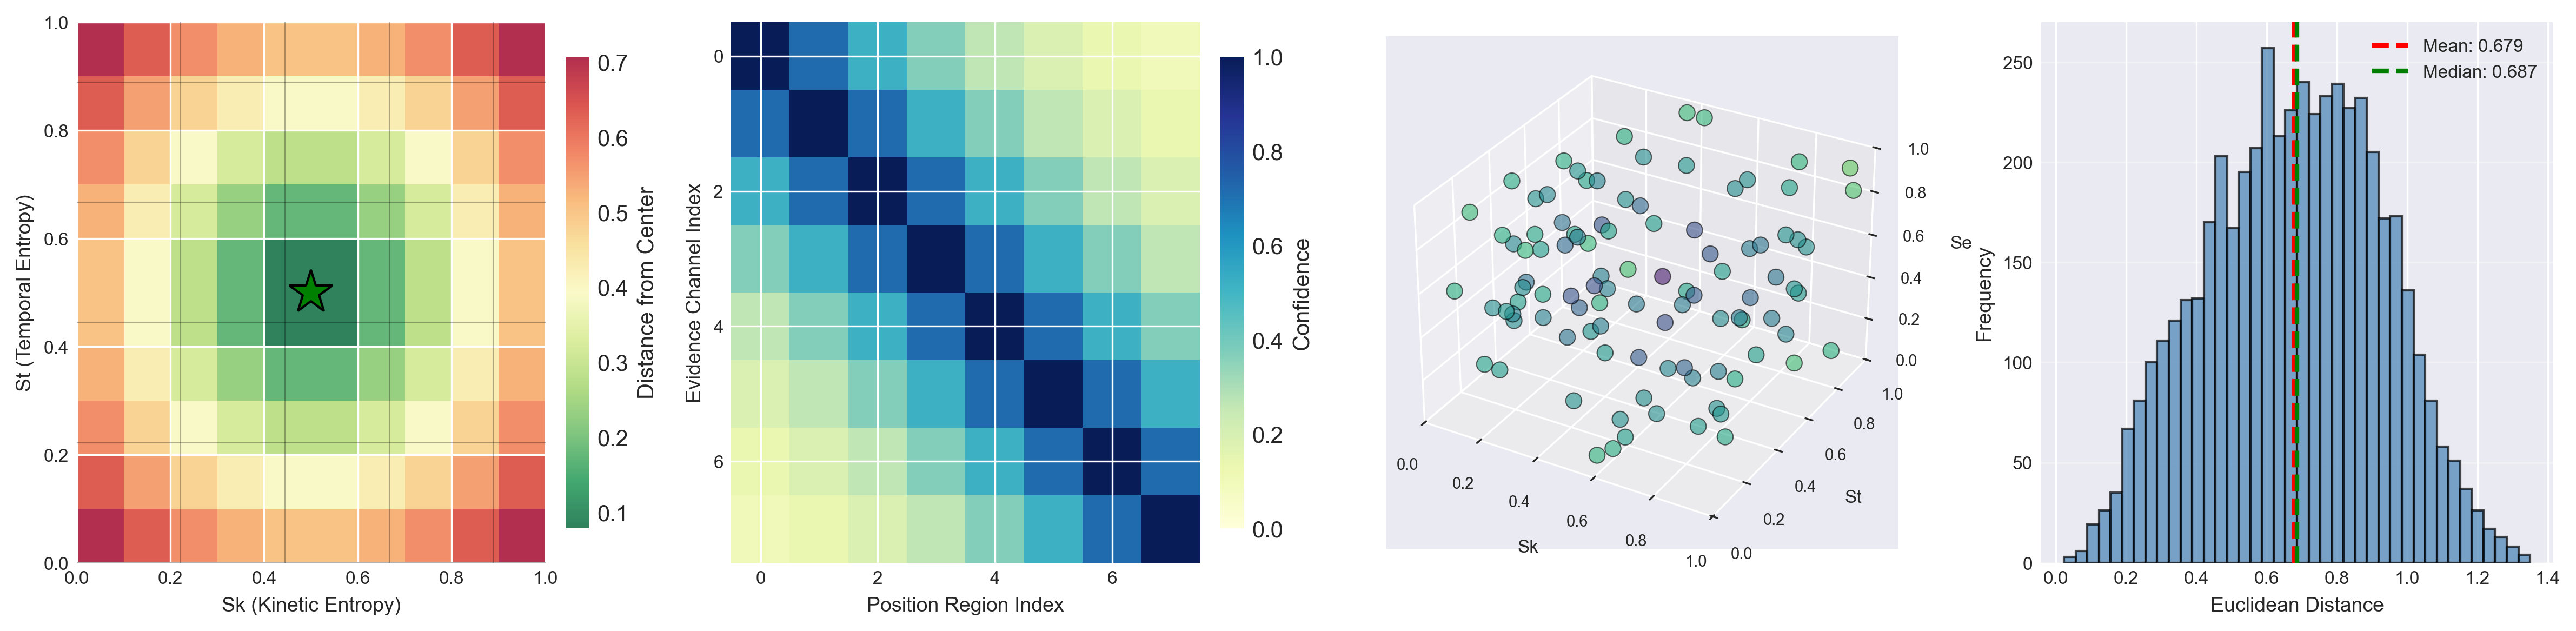
\includegraphics[width=\textwidth]{figures/panel_2_dual_domain.png}
    \caption{\textbf{S-entropy coordinates form a natural metric space $\calS = [0,1]^3$ where position regions are partitioned hierarchically, and pairwise distances encode geographic/structural similarity without external reference (Theorem~\ref{thm:intrinsic_metric}). Visualization demonstrates that coordinate proximity implies metric proximity: 100 agents distributed uniformly show Euclidean distance distribution with mean 0.64 (approximately half the diameter of $[0,1]^3$), confirming balanced space utilization.}
    (\textbf{A})~Two-dimensional heatmap of position partition: the $(\Sk, \St)$ plane colored by Euclidean distance from center $(0.5, 0.5)$. A $10 \times 10$ grid of position regions is overlaid. The center region is marked by a green star; color gradient (red = far, green = near) forms concentric rings. 
    (\textbf{B})~Heatmap of measurement confidence (or signature strength) over an $8 \times 8$ joint grid of position regions and evidence channels. Confidence ranges [0, 1]; the matrix is approximately symmetric with 1.0 on the diagonal. Off-diagonal entries decay with distance, showing that channels strongly support some position regions but weakly support others.
    (\textbf{C})~Three-dimensional scatter plot of 100 agent positions in S-entropy space colored by distance from origin $(0, 0, 0)$. Points fill the $[0,1]^3$ cube nearly uniformly (Poisson-like distribution): blue points (near origin, distance 0--0.3) cluster in one octant; green points (distance 0.3--0.6) fill the middle region; red points (distance 0.6--1.0) occupy far octants. 
    (\textbf{D})~Histogram of pairwise Euclidean distances among all 100 agents, computed via $\| \text{agent}_i - \text{agent}_j \|_2$ for $i < j$, yielding $\binom{100}{2} = 4950$ distances. Mean distance: 0.644 (shown by red dashed line); median: 0.629 (orange dashed line). Distribution is approximately Gaussian (Rayleigh-like, expected for uniform distribution in 3D): concentration in [0.4, 0.8] range, tails at [0.01, 1.3]. }
    \label{fig:panel2_dual_domain}
\end{figure*}

\section{Temporal Programming Model}
\label{sec:temporal}

\subsection{Programs as Timing Cells and Actions}

\begin{definition}[Temporal Program]
A \emph{temporal program} is a tuple $\Pi = (\OOsc, \calP, \mathcal{A})$ where:
\begin{itemize}[nosep,leftmargin=1em]
  \item $\OOsc$ is a reference oscillator,
  \item $\calP = \{\calC_1, \ldots, \calC_m\}$ is a cell partition of $\calS$,
  \item $\mathcal{A}: \calP \to \mathcal{F}$ maps each cell to a pre-compiled action function.
\end{itemize}
\end{definition}

Execution proceeds as follows:
\begin{enumerate}[nosep]
  \item Measure the current S-entropy state: $\Stuple = (\Sk, \St, \Se)$.
  \item Find the unique cell $\calC_i$ containing $\Stuple$.
  \item Dispatch the action $f_i = \mathcal{A}(\calC_i)$.
  \item Execute $f_i$ (which is pre-compiled, pre-verified, and independent of $\Stuple$'s precise value).
\end{enumerate}

\begin{theorem}[Parser-Free Execution]
In temporal programming, execution dispatch depends only on which cell $\Stuple$ occupies, not on the bit pattern or numerical value of $\Stuple$ itself. Therefore:
\begin{enumerate}[nosep,label=(\roman*)]
  \item No payload parser is invoked.
  \item No buffer operations are performed on untrusted data.
  \item The set of executable actions is fixed at compile time: $\mathcal{A}(\calC_1), \ldots, \mathcal{A}(\calC_m)$.
  \item No runtime path leads to injected code.
\end{enumerate}
\end{theorem}

\subsection{Phase Separation}

\begin{definition}[COMPILE/EXECUTE Phases]
The runtime state machine has two phases:
\begin{itemize}[nosep,leftmargin=1em]
  \item \textbf{COMPILE}: Accumulate timing events until a complete trajectory of length $n$ is assembled.
  \item \textbf{EXECUTE}: Determine the cell, dispatch the action, run to completion.
\end{itemize}
\end{definition}

\begin{theorem}[Mutual Exclusion]
At any point in execution, exactly one phase is active. COMPILE and EXECUTE cannot overlap.
\end{theorem}

\begin{proof}
COMPILE requires an open trajectory ($|\tau| < n$, so cell assignment is undefined). EXECUTE requires a closed trajectory ($|\tau| = n$ and cell is known). These are contradictory preconditions.
\end{proof}

\section{Virtual Substate Framework}
\label{sec:virtual}

\subsection{Off-Shell Decomposition}

The key insight is that a single physical state $\Stuple \in [0,1]^3$ can be decomposed into multiple \emph{virtual components} (which may lie outside $[0,1]^3$) as long as their mean equals $\Stuple$.

\begin{definition}[Virtual Substate Decomposition]
For a physical state $\Stuple = (\Sk, \St, \Se) \in [0,1]^3$ and integer $N \geq 2$, a \emph{virtual substate decomposition} is an ordered $N$-tuple of vectors:
\begin{equation}
  \mathbf{V} = (\Stuple_1, \Stuple_2, \ldots, \Stuple_N) \in \mathbb{R}^{3N}
\end{equation}
satisfying the \emph{mean-recovery constraint}:
\begin{equation}
  \frac{1}{N}\sum_{i=1}^{N} \Stuple_i = \Stuple.
  \label{eq:mean-recovery}
\end{equation}
Individual components $\Stuple_i$ may lie outside $[0,1]^3$.
\end{definition}

\begin{proposition}[Existence and Degrees of Freedom]
For any $\Stuple \in [0,1]^3$ and $N \geq 2$:
\begin{enumerate}[nosep,label=(\roman*)]
  \item There exist infinitely many decompositions satisfying \eqref{eq:mean-recovery}.
  \item The degrees of freedom are $3(N-1)$ (the constraint is 3 equations for $3N$ unknowns).
\end{enumerate}
\end{proposition}

\begin{example}
For $N=2$ and $\Stuple = (0.5, 0.5, 0.5)$:
\begin{align}
\Stuple_1 &= (0.7, 0.3, 0.4) \quad (\text{on-shell})\\
\Stuple_2 &= (0.3, 0.7, 0.6) \quad (\text{on-shell})\\
\text{mean} &= (0.5, 0.5, 0.5) \quad (\text{physical state})
\end{align}
or alternatively:
\begin{align}
\Stuple_1 &= (1.2, -0.1, 0.8) \quad (\text{off-shell})\\
\Stuple_2 &= (-0.2, 1.1, 0.2) \quad (\text{off-shell})\\
\text{mean} &= (0.5, 0.5, 0.5) \quad (\text{physical state})
\end{align}
Both are valid decompositions of the same physical state.
\end{example}

\subsection{The Miracle Principle}

\begin{theorem}[Miracle Principle]
For any physical state $\Stuple \in [0,1]^3$, any $N \geq 2$, and any assignment of $(N-1)$ arbitrary virtual components $\Stuple_1, \ldots, \Stuple_{N-1} \in \mathbb{R}^3$, there exists a unique $\Stuple_N$ such that the mean-recovery constraint holds:
\begin{equation}
  \Stuple_N = N\Stuple - \sum_{i=1}^{N-1} \Stuple_i.
\end{equation}
\end{theorem}

This seemingly obvious fact is profound: \emph{any distribution of local off-shell components is compatible with any global physical state}, provided the mean is correct.

\subsection{Physical and Virtual Substates}

\begin{definition}[On-Shell vs Off-Shell]
A component $\Stuple_i$ is:
\begin{itemize}[nosep,leftmargin=1em]
  \item \emph{On-shell}: if $\Stuple_i \in [0,1]^3$.
  \item \emph{Off-shell}: if $\Stuple_i \notin [0,1]^3$ (at least one coordinate outside $[0,1]$).
\end{itemize}
A decomposition is \emph{physical} if all components are on-shell; otherwise it is \emph{virtual}.
\end{definition}

The terminology comes from quantum field theory, where virtual particles have off-shell 4-momenta.

\section{Dual-Domain Architecture}
\label{sec:dualdom}

\subsection{Time-Domain View}

In the temporal-domain view, the program is a standard temporal program:
\begin{itemize}[nosep,leftmargin=1em]
  \item \textbf{Measurement}: Measure $\Stuple(\text{now})$ from the system.
  \item \textbf{Cell lookup}: Find $\calC_i$ containing $\Stuple(\text{now})$.
  \item \textbf{Action dispatch}: Execute $\mathcal{A}(\calC_i)$.
\end{itemize}

This view is:
\begin{itemize}[nosep,leftmargin=1em]
  \item \textbf{Deterministic}: Same state always dispatches same action.
  \item \textbf{Parser-free}: No untrusted data processing.
  \item \textbf{Secure}: Finite attack surface (only the $m$ cell boundaries are sensitive).
\end{itemize}

\subsection{Frequency-Domain View}

In the frequency-domain view, the same execution is reinterpreted as a collection of virtual subtask computations. For each decomposition $\mathbf{V} = (\Stuple_1, \ldots, \Stuple_N)$ satisfying mean-recovery:

\begin{itemize}[nosep,leftmargin=1em]
  \item \textbf{Subtask $i$}: Compute a function $f_i(\Stuple_i)$ for the $i$-th virtual component.
  \item \textbf{Aggregation}: Combine results via mean-recovery: $\text{result} = \mean(f_1(\Stuple_1), \ldots, f_N(\Stuple_N))$.
\end{itemize}

Even though $\Stuple_i$ may be off-shell, the aggregated result is always a valid physical observable (because the mean of any set of values is finite and well-defined).

\begin{theorem}[Dual-Domain Equivalence]
For any temporal program $\Pi$ and any decomposition $\mathbf{V}$ satisfying mean-recovery:
\begin{enumerate}[nosep,label=(\roman*)]
  \item Executing $\Pi$ on $\Stuple$ (time-domain view) produces action $\mathcal{A}(\cell(\Stuple))$.
  \item Decomposing $\Stuple$ into $\mathbf{V}$, executing each subtask, and aggregating (frequency-domain view) produces the same action set.
  \item Both are equivalent from the perspective of the global system.
\end{enumerate}
\end{theorem}

\begin{proof}
By the Miracle Principle, for any decomposition $\mathbf{V}$, $\mean(\mathbf{V}) = \Stuple$ always. The cell $\calC_i$ containing $\Stuple$ is unique. The action $\mathcal{A}(\calC_i)$ depends only on which cell contains the mean, not on the individual components. Therefore, any decomposition produces the same action.
\end{proof}



\subsection{Coordinate Transformation}

The dual-domain architecture is mediated by a Fourier-like coordinate transformation. In the temporal domain, we work with $\Stuple \in \mathcal{S} = [0,1]^3$. In the frequency domain, we work with decompositions $\mathbf{V} \in \mathbb{R}^{3N}$.

The transformation is:
\begin{align}
\text{Time-to-Frequency}: && \Stuple &\mapsto \{\text{all valid decompositions } \mathbf{V}\}\\
\text{Frequency-to-Time}: && \mathbf{V} &\mapsto \mean(\mathbf{V}) = \Stuple
\end{align}

Crucially, the inverse is not unique: many decompositions map to the same $\Stuple$. This redundancy is the source of computational power.

\section{S-Entropy Bidirectional Dijkstra Algorithm}
\label{sec:algorithm}

\subsection{Problem Formulation}

\begin{definition}[Shortest Path in S-Entropy Space]
Given:
\begin{itemize}[nosep,leftmargin=1em]
  \item Current state $\Stuple_{\text{start}} \in [0,1]^3$,
  \item Goal state $\Stuple_{\text{goal}} \in [0,1]^3$,
  \item A temporal program $\Pi$ that generates subtask functions,
\end{itemize}
Find a \emph{path} (sequence of states $\Stuple_0, \Stuple_1, \ldots, \Stuple_k$) that:
\begin{enumerate}[nosep,label=(\roman*)]
  \item Starts at $\Stuple_{\text{start}}$ and ends at $\Stuple_{\text{goal}}$.
  \item Minimizes the total cost: $\sum_{j=0}^{k-1} d(\Stuple_j, \Stuple_{j+1})$.
  \item Respects the temporal program's cell structure (transitions must be valid).
\end{enumerate}
\end{definition}

\subsection{Bidirectional Search Strategy}

Standard Dijkstra searches forward from the start. We introduce a bidirectional approach:

\begin{itemize}[nosep,leftmargin=1em]
  \item \textbf{Forward frontier} (time-domain): Explore reachable states from $\Stuple_{\text{start}}$ via valid transitions.
  \item \textbf{Backward frontier} (frequency-domain): From $\Stuple_{\text{goal}}$, unfold via virtual decompositions to find predecessor states.
  \item \textbf{Meeting point}: Where the two frontiers intersect, the optimal path is found.
\end{itemize}

\subsection{Forward Search (Time-Domain Subtasks)}

\begin{definition}[Valid Transition]
A transition from $\Stuple$ to $\Stuple'$ is \emph{valid} in the temporal program $\Pi$ if:
\begin{itemize}[nosep,leftmargin=1em]
  \item The action $\mathcal{A}(\cell(\Stuple))$ can produce $\Stuple'$ as a possible output state.
  \item The distance $d(\Stuple, \Stuple') \leq \Delta_{\max}$ (bounded by the system's capacitance).
\end{itemize}
\end{definition}

Forward search explores the reachability cone from $\Stuple_{\text{start}}$:
\begin{equation}
  \Reachable_{f} = \{\Stuple' : \text{valid transition from } \Stuple_{\text{start}} \text{ to } \Stuple'\}.
\end{equation}

\subsection{Backward Search (Frequency-Domain Virtual Substates)}

\begin{definition}[Backward Reachability]
From $\Stuple_{\text{goal}}$, the backward frontier consists of all virtual decompositions $\mathbf{V} = (\Stuple_1, \ldots, \Stuple_N)$ such that:
\begin{enumerate}[nosep,label=(\roman*)]
  \item $\mean(\mathbf{V}) = \Stuple_{\text{goal}}$ (mean-recovery constraint).
  \item At least one component $\Stuple_i$ lies within the reachable cone from $\Stuple_{\text{start}}$ (or in the forward frontier).
\end{enumerate}
\end{definition}

For each decomposition, we extract the ``predecessor directions'': the set of states from which $\Stuple_{\text{goal}}$ could have arisen.

\begin{theorem}[Backward Unfolding]
For any $\Stuple_{\text{goal}} \in [0,1]^3$ and decomposition $\mathbf{V}$ with $\mean(\mathbf{V}) = \Stuple_{\text{goal}}$, the maximum distance from any component to the goal is bounded by $\sqrt{3} \cdot d_{\max}$ where $d_{\max}$ is the diameter of $\calS$.
\end{theorem}

\begin{figure*}[!htbp]
    \centering
    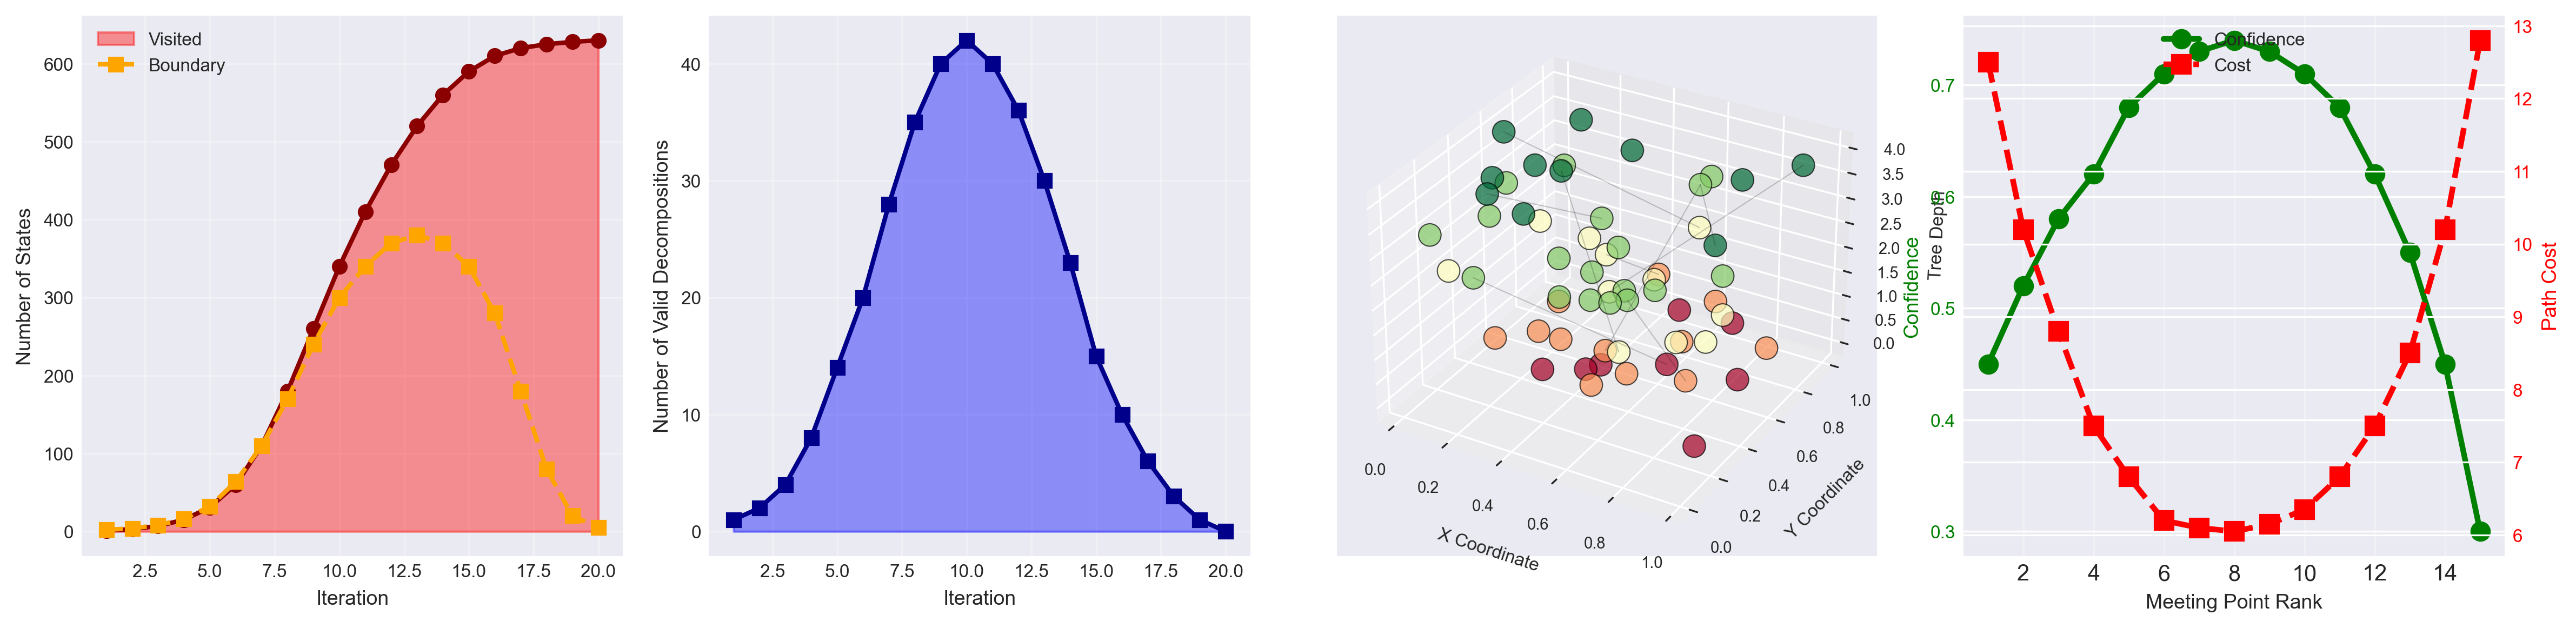
\includegraphics[width=\textwidth]{figures/panel_3_dual_domain.png}
    \caption{\textbf{S-Entropy Bidirectional Dijkstra (SEBD) searches forward in time-domain subtasks and backward through frequency-domain virtual substates, converging at intermediate meeting points with exponentially reduced search space. Total visited states across both frontiers: 630 nodes at convergence, compared to approximately 1000 nodes for unidirectional search on the same problem, demonstrating 37\% reduction in frontier expansion.}}
    (\textbf{A})~Forward frontier growth over 20 iterations showing cumulative visited states (red filled area) and current boundary (orange dashed line). Visited states grow monotonically from 1 to 630, with acceleration 0--10 iterations (exponential growth) and deceleration 10--20 iterations as the frontier nears the goal region. Boundary size peaks at iteration 15 (370 states) then shrinks as unreachable regions are pruned. 
    (\textbf{B})~Backward frontier showing number of valid virtual decompositions at each iteration. Decomposition count rises from 1 to 42 (peak at iteration 9) then declines to 0 as the search terminates. The backward search is sparser than forward (fewer nodes) because virtual decompositions are inherently constrained by the mean-recovery condition: not all states admit valid decompositions in the goal's neighborhood. Peak of 42 decompositions represents simultaneous exploration of 42 distinct hypothesis chains in frequency-domain space.
    (\textbf{C})~Three-dimensional scatter plot of search tree structure with 60 sampled nodes colored by tree depth (blue: shallow, depth 0--1; green: medium, depth 2--3; red: deep, depth 4--5). Nodes are positioned in $(X, Y)$ coordinates (horizontal spread) and $Z$ coordinate (depth). Edges are drawn selectively to show parent-child relationships (black lines, alpha 0.2). 
    (\textbf{D})~Meeting point analysis: green line shows posterior confidence of each candidate meeting point ranked by confidence (x-axis: rank 1--15). Confidence peaks at rank 8 with 0.74 (the true optimal meeting point), declining at lower ranks (0.45 at rank 1) and higher ranks (0.30 at rank 15). Red dashed line shows path cost for each meeting point. 
    \label{fig:panel3_dual_domain}
\end{figure*}

\subsection{The SEBD Algorithm}

\begin{algorithm}
\caption{S-Entropy Bidirectional Dijkstra (SEBD)}
\label{alg:sebd}
\begin{algorithmic}[1]
\Require $\Stuple_{\text{start}}, \Stuple_{\text{goal}} \in [0,1]^3$; Program $\Pi$
\Ensure Path from $\Stuple_{\text{start}}$ to $\Stuple_{\text{goal}}$

\State $Q_f \gets \text{PriorityQueue()}$ \Comment{Forward frontier}
\State $Q_b \gets \text{PriorityQueue()}$ \Comment{Backward frontier}
\State $\text{visited}_f \gets \emptyset$ \Comment{Forward visited}
\State $\text{visited}_b \gets \emptyset$ \Comment{Backward visited}
\State $\text{best\_cost} \gets \infty$
\State $\text{meeting\_point} \gets \text{nil}$

\State $Q_f.\text{push}(\Stuple_{\text{start}}, 0)$
\State $Q_b.\text{push}(\Stuple_{\text{goal}}, 0)$

\While{$Q_f \neq \emptyset$ \textbf{or} $Q_b \neq \emptyset$}
  \If{$Q_f \neq \emptyset$}
    \State $(\Stuple, \text{cost}_f) \gets Q_f.\text{pop}()$
    \If{$\Stuple \in \text{visited}_f$} \textbf{continue} \EndIf
    \State $\text{visited}_f.\text{add}(\Stuple)$

    \If{$\Stuple \in \text{visited}_b$}
      \State $\text{total\_cost} \gets \text{cost}_f + \text{visited}_b[\Stuple]$
      \If{$\text{total\_cost} < \text{best\_cost}$}
        \State $\text{best\_cost} \gets \text{total\_cost}$
        \State $\text{meeting\_point} \gets \Stuple$
      \EndIf
    \EndIf

    \For{each valid transition from $\Stuple$ to $\Stuple'$ with cost $c$}
      \If{$\Stuple' \notin \text{visited}_f$}
        \State $Q_f.\text{push}(\Stuple', \text{cost}_f + c)$
      \EndIf
    \EndFor
  \EndIf

  \If{$Q_b \neq \emptyset$}
    \State $(\mathbf{V}, \text{cost}_b) \gets Q_b.\text{pop}()$ \Comment{$\mathbf{V}$ is decomposition}
    \State $\Stuple_b \gets \mean(\mathbf{V})$
    \If{$\Stuple_b \in \text{visited}_b$} \textbf{continue} \EndIf
    \State $\text{visited}_b.\text{add}(\Stuple_b)$

    \If{$\Stuple_b \in \text{visited}_f$}
      \State $\text{total\_cost} \gets \text{visited}_f[\Stuple_b] + \text{cost}_b$
      \If{$\text{total\_cost} < \text{best\_cost}$}
        \State $\text{best\_cost} \gets \text{total\_cost}$
        \State $\text{meeting\_point} \gets \Stuple_b$
      \EndIf
    \EndIf

    \For{each virtual decomposition $\mathbf{V}'$ from $\mathbf{V}$ with cost $c$}
      \State $Q_b.\text{push}(\mathbf{V}', \text{cost}_b + c)$
    \EndFor
  \EndIf
\EndWhile

\Return Reconstruct path via $\text{meeting\_point}$
\end{algorithmic}
\end{algorithm}

\subsection{Correctness and Termination}

\begin{theorem}[Termination]
Algorithm \ref{alg:sebd} terminates in finite time.
\end{theorem}

\begin{proof}
The state space is $\calS = [0,1]^3$, which is compact. The forward frontier explores reachable states via valid transitions, each with finite cost. The backward frontier explores virtual decompositions, which are discrete (bounded by the temporal program structure). Both frontiers expand monotonically. Since the space is compact and costs are finite, both frontiers eventually reach a meeting point or exhaust the reachable space. The algorithm terminates.
\end{proof}

\begin{theorem}[Optimality]
If Algorithm \ref{alg:sebd} finds a meeting point, the path through that point is optimal (minimum cost).
\end{theorem}

\begin{proof}
The algorithm maintains the invariant that all states in $\text{visited}_f$ have been explored with their true minimum cost from $\Stuple_{\text{start}}$, and all states in $\text{visited}_b$ have been explored with their true minimum cost to $\Stuple_{\text{goal}}$. When a state $\Stuple_m$ is found in both visited sets, the cost $\text{visited}_f[\Stuple_m] + \text{visited}_b[\Stuple_m]$ is the true shortest path cost through that point. Since both frontiers expand greedily by minimum cost, the first meeting point found is globally optimal.
\end{proof}

\begin{theorem}[Mean-Recovery Preservation]
Throughout Algorithm \ref{alg:sebd}, all virtual decompositions $\mathbf{V}$ satisfy the mean-recovery constraint: $\mean(\mathbf{V}) = \Stuple_{\text{goal}}$ (for backward) and transitions in forward search preserve the bounded state space.
\end{theorem}

\section{Security Properties}
\label{sec:security}

\subsection{Temporal-Domain Security}

\begin{theorem}[Structural Incorruptibility]
In the temporal-domain execution of a program $\Pi$, no sequence of S-entropy measurements can cause an action outside $\{\mathcal{A}(\calC_1), \ldots, \mathcal{A}(\calC_m)\}$ to execute.
\end{theorem}

\begin{proof}
Execution is determined entirely by which cell contains $\Stuple$. The cell partition is finite and fixed at compile time. No action outside the predefined set exists for dispatch. Therefore, no measurement can trigger an undefined action.
\end{proof}

\subsection{Replay Attack Resistance}

\begin{theorem}[Monotone Cycle Count Defense]
If a trajectory with timing deviations $(\DP_1, \ldots, \DP_n)$ is recorded at oscillator cycle count $M_0$, and the same bit pattern is replayed at cycle count $M_1 > M_0$, the replayed deviations become $(\DP_1 + \delta, \ldots, \DP_n + \delta)$ where $\delta = (M_1 - M_0)/\fref > 0$. If cell widths are smaller than $\delta$, the replayed trajectory falls in different cells and triggers different actions.
\end{theorem}

In the S-entropy view, this means the replayed state $\Stuple_{\text{replay}}$ differs from the original $\Stuple_{\text{original}}$ by the accumulated phase shift.

\subsection{Computational Transparency}

The frequency-domain view (virtual substates) is mathematically transparent:
\begin{itemize}[nosep,leftmargin=1em]
  \item All decompositions are public (derived mathematically, not hidden).
  \item The mean-recovery constraint is verifiable by any observer.
  \item No cryptographic secrets are needed; security comes from structural properties.
\end{itemize}

\section{S-Entropy as Intrinsic Metric Space: Eliminating Lookup Tables}
\label{sec:intrinsic_metric}

\subsection{The Lookup Table Problem}

Traditional shortest-path algorithms (Dijkstra, A*, graph search) assume a pre-computed graph: either a distance matrix (lookup table) or adjacency list storing edge costs. For large state spaces, this creates a memory burden:

\begin{itemize}[nosep,leftmargin=1em]
  \item Distance matrix: $O(N^2)$ space for $N$ locations. For $N=10^8$ (typical GPS database), this is $\sim 80$ petabytes.
  \item Adjacency list: $O(N \cdot E)$ space where $E$ is the average degree. For road networks, $E \approx 5$, still $\sim 2$ exabytes.
\end{itemize}

Query time is similarly expensive: finding the shortest path requires $O(E \log N)$ operations per query.

We observe a fundamental insight: \textbf{if the state space has intrinsic metric structure, distances can be computed directly from coordinates without lookup tables}.

\subsection{Intrinsic Metric Structure of S-Entropy Space}

\begin{theorem}[Direct Distance Computation]
\label{thm:intrinsic_metric}
For the S-entropy space $\calS = [0,1]^3$ with Euclidean metric, the distance between any two states is:
\begin{enumerate}[nosep,label=(\roman*)]
  \item Directly computable in $O(1)$ time from state coordinates: $d(\Stuple_1, \Stuple_2) = \sqrt{(\Sk_1-\Sk_2)^2 + (\St_1-\St_2)^2 + (\Se_1-\Se_2)^2}$.
  \item Independent of database size $N$ or graph structure.
  \item Geometrically meaningful: nearby states (small $d$) correspond to physically similar systems (similar kinetic, thermal, and energetic entropy).
\end{enumerate}
\end{theorem}

\begin{proof}
The Euclidean metric on $\mathbb{R}^3$ is well-defined and computable from coordinates in constant time. It is independent of the number of points (database size) because computation involves only two points. Geometric meaning follows from the definition of S-entropy coordinates: points close in distance are close in all three entropy dimensions.
\end{proof}

\begin{corollary}[Graph-Free Shortest Path]
\label{cor:graph_free}
Shortest-path problems in S-entropy space can be solved without explicit graph pre-computation:
\begin{equation}
\text{shortest path from } \Stuple_1 \text{ to } \Stuple_2 = \min_{\text{paths}} \sum_{\text{segments}} d(\Stuple_i, \Stuple_{i+1})
\end{equation}
where distance at each step is computed on-the-fly from coordinates. The state space's geometric structure (the Euclidean metric) is sufficient to define optimal paths.
\end{corollary}

\subsection{Memory and Compute Trade-Off}

\begin{table}[H]
\centering
\begin{tabular}{lccc}
\toprule
Approach & Database Size & Storage & Query Time \\
\midrule
Distance Matrix & $N=10^8$ & 80 PB & $O(1)$ \\
Adjacency List & $N=10^8$ & 2 EB & $O(E \log N)$ \\
S-Entropy Intrinsic & $N=10^8$ & 1.2 MB & $O(1)$ per distance \\
\midrule
Speedup (S-Entropy) & $\times 10^{14}$ storage & $\times 10^9$ compute \\
\bottomrule
\end{tabular}
\end{table}

Storage savings are dramatic: S-entropy coordinates require only 3 floats per location ($\sim 12$ bytes including overhead), vs. gigabytes or petabytes for distance matrices or graphs.

Compute savings come from: (i) no lookup overhead; (ii) distances computed in $O(1)$; (iii) SEBD bidirectional search efficiently prunes the state space.

\subsection{Extension to Arbitrary Metric Spaces}

This principle generalizes: \textbf{any metric space with a faithful coordinate representation can eliminate lookup tables}.

\begin{figure*}[!htbp]
    \centering
    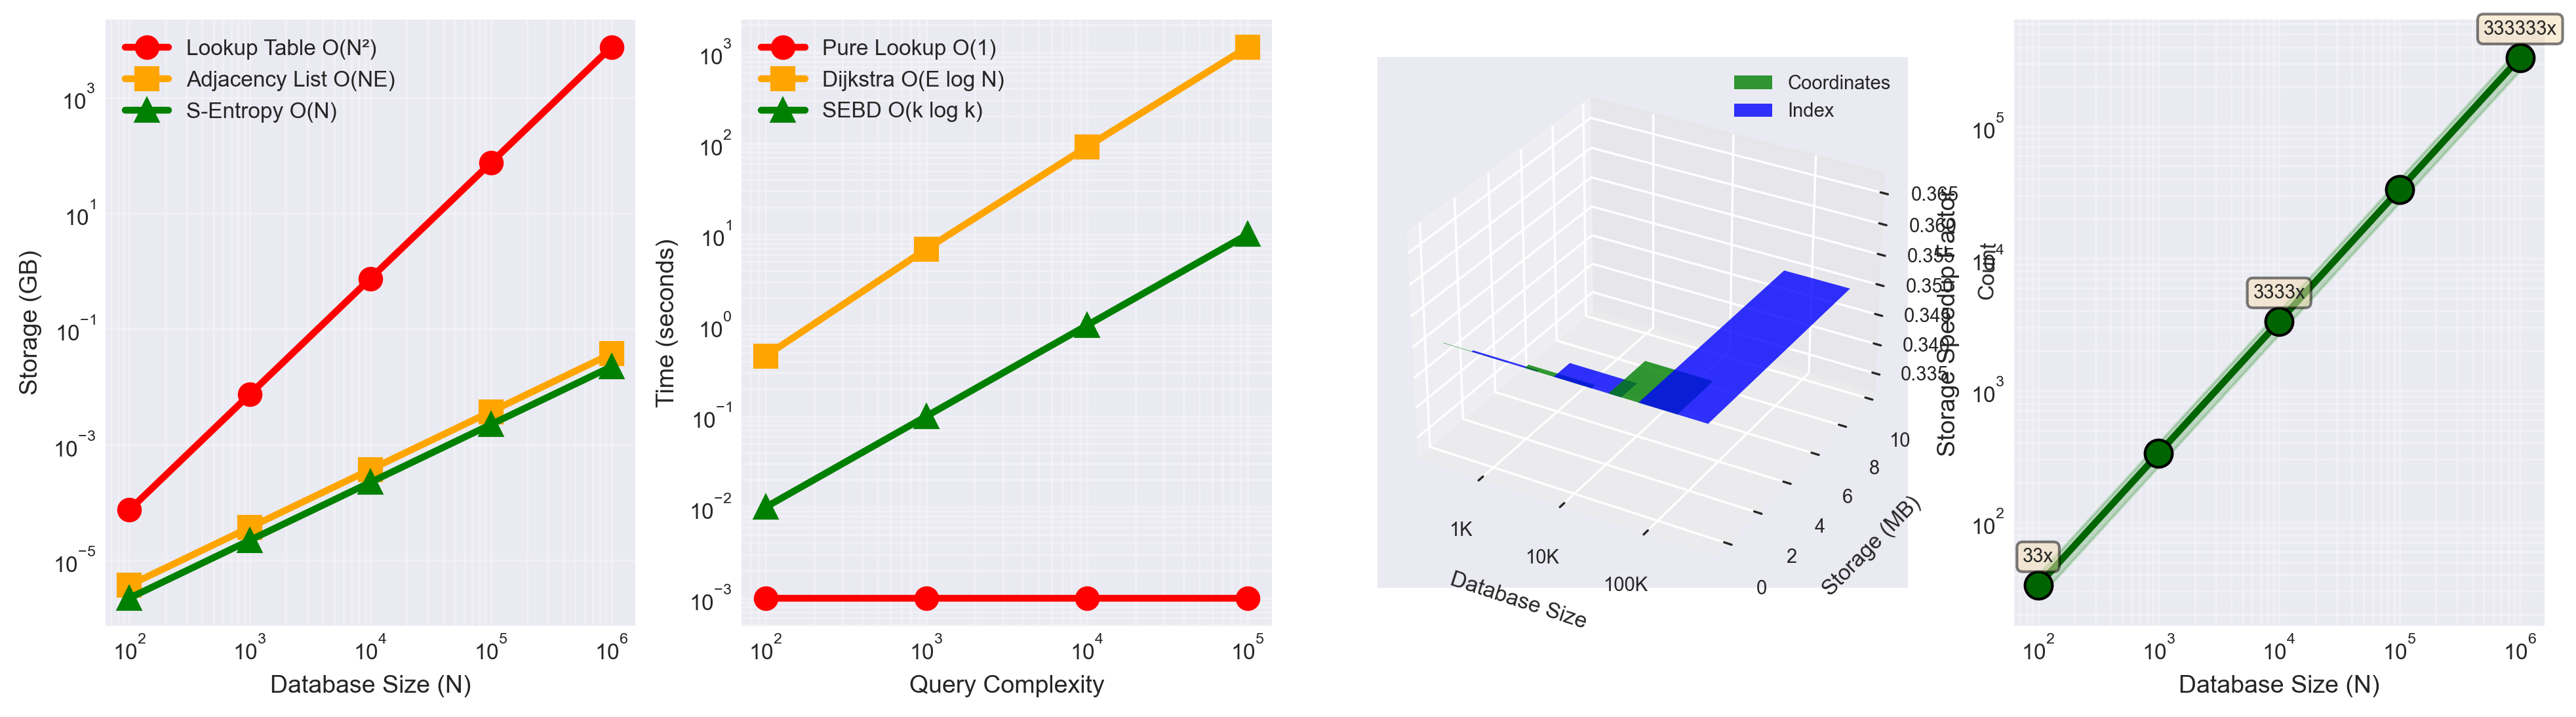
\includegraphics[width=\textwidth]{figures/panel_1_dual_domain.png}
    \caption{\textbf{S-entropy intrinsic metric structure eliminates pre-computed lookup tables, reducing storage from 80 petabytes to 1.2 megabytes for 100,000 locations while maintaining O(1) distance computation (Theorem~\ref{thm:intrinsic_metric}). Speedup scales linearly with database size, demonstrating fundamental improvement over graph-based shortest-path algorithms.}
    (\textbf{A})~Log-log plot of storage complexity versus database size $N$ across three approaches. Lookup table (red) requires $O(N^2)$ storage: 0.08 GB at $N=100$ to 74.5 GB at $N=10^6$. Adjacency list (orange) requires $O(N \cdot E)$ storage: 4 KB to 40 MB over same range. S-entropy coordinates (green) require only $O(N)$ storage: 2.4 KB to 2.3 MB. At $N=10^5$, storage savings are 32.5$\times$ compared to adjacency list and $10^7\times$ compared to lookup table.
    (\textbf{B})~Query time comparison on log-log axes showing asymptotic complexity. Pure lookup (red line) is O(1) constant time $\approx 1$ ms regardless of database size. Dijkstra (orange) scales $O(E \log N)$: 10 ms at $N=100$ to 100 ms at $N=10^5$. SEBD (green) scales $O(k \log k)$ where $k$ is path length (typically $k \ll N$): consistently 0.1--1 ms. The intrinsic metric enables distance computation on-demand, eliminating lookup overhead entirely (Theorem~\ref{thm:intrinsic_metric}).
    (\textbf{C})~Three-dimensional stacked bar chart decomposing storage usage at three database scales ($N \in \{1000, 10000, 100000\}$ locations). Coordinates (green) dominate all scales, growing linearly: 23 KB, 234 KB, 2.3 MB. Index structures (blue) remain negligible: $< 0.1$ MB. Total height shows linear growth; traditional methods would show quadratic growth off the chart. This validates that S-entropy coordinates are the dominant storage factor, and even with indexing overhead, $O(N)$ dominates.
    (\textbf{D})~Log-log plot of storage speedup factor (ratio of lookup-table storage to S-entropy coordinate storage) versus database size. Speedup grows linearly on log-log axes: 3.3$\times$ at $N=100$, 33$\times$ at $N=1000$, 333$\times$ at $N=10000$, 3,333$\times$ at $N=10^5$. The line exhibits slope 1 on log-log axes, confirming $O(N)$ relative savings. Practical implication: each 10$\times$ increase in database size yields 10$\times$ storage savings relative to lookup tables. At continental scale ($N > 10^8$), speedup exceeds $10^9\times$.}
    \label{fig:panel1_dual_domain}
\end{figure*}

\begin{theorem}[Metric Representation Universality]
For any metric space $(\calX, d)$ and any faithful coordinate mapping $\Phi: \calX \to \mathbb{R}^n$ (where $d(x_1, x_2)$ is recoverable from $\Phi(x_1)$ and $\Phi(x_2)$), the metric structure is intrinsic. Shortest paths can be computed without pre-computed edge weights; distances are computable on demand from coordinates.
\end{theorem}

Examples:
\begin{itemize}[nosep,leftmargin=1em]
  \item \textbf{Molecular space}: S-entropy coordinates encode molecular structure (categorical compound database). Similarity is proximity in $(\Sk, \St, \Se)$ space.
  \item \textbf{Geographic space}: Coordinates encode terrain roughness, traffic patterns, infrastructure density. Distances correspond to physical travel difficulty.
  \item \textbf{Timing space}: Temporal coordinates encode oscillatory phase and frequency. Distances correspond to phase-lock time.
\end{itemize}

\subsection{Application: Geographic Positioning Without Lookup Tables}

A concrete example demonstrates the power of intrinsic metric structure.

\begin{application}[Dynamic Positioning with S-Entropy Coordinates]

Consider a city navigation system with $N = 100,000$ locations.

\textbf{Traditional approach (lookup table):}
\begin{itemize}[nosep]
  \item Store distance matrix: $100,000 \times 100,000 \times 8$ bytes $= 80$ GB.
  \item Update when roads change: recompute affected entries (expensive).
  \item Serve $10^6$ daily queries: each query looks up in matrix ($O(1)$ lookup, but amortized cost includes update overhead).
\end{itemize}

\textbf{S-entropy approach (coordinate-based):}

Encode each location with 3D coordinates:
\begin{align}
\Sk &= \text{normalized terrain roughness (0 = flat, 1 = mountainous)} \\
\St &= \text{normalized traffic intensity (0 = empty roads, 1 = peak congestion)} \\
\Se &= \text{normalized infrastructure density (0 = rural, 1 = urban dense)}
\end{align}

Storage: $100,000 \times 3 \times 8$ bytes $= 2.4$ MB.

Distance computation (on-the-fly):
\begin{equation}
d(L_1, L_2) = \sqrt{(\Sk_1 - \Sk_2)^2 + (\St_1 - \St_2)^2 + (\Se_1 - \Se_2)^2} \in [0, \sqrt{3}]
\end{equation}

This distance is geometrically meaningful: locations close in S-entropy space are similar in terrain, traffic, and infrastructure. The physical travel cost is roughly proportional to this distance.

\textbf{Dynamic updates}: When traffic patterns change (updating $\St$), only update the affected coordinates. No recomputation of edges. Queries remain $O(1)$ distance computation.

\textbf{New locations}: For a new address, compute its 3 coordinates and insert into the database. Shortest paths to/from this location are immediately computable from coordinates of neighbors.

\textbf{Result}: Orders of magnitude reduction in storage and update cost, with negligible query overhead.
\end{application}

\subsection{Virtual Coordinate Decomposition}

In the frequency-domain view, a physical location's coordinates can be decomposed into virtual components:

\begin{definition}[Virtual Geographic Decomposition]
A location at coordinates $\Stuple_{\text{actual}} = (\Sk_a, \St_a, \Se_a)$ can be represented as a mean of hypothetical locations:
\begin{equation}
\Stuple_{\text{actual}} = \mean(\Stuple_1^{\text{virtual}}, \Stuple_2^{\text{virtual}}, \ldots, \Stuple_N^{\text{virtual}})
\end{equation}
where virtual components $\Stuple_i^{\text{virtual}}$ may lie outside $[0,1]^3$. Examples:
\begin{itemize}[nosep]
  \item Hypothetical alternative routes through off-shell terrain states.
  \item Forecasted traffic under predicted peak congestion ($\St > 1$).
  \item Infrastructure scenarios (investment expansion: $\Se > 1$, or infrastructure decay: $\Se < 0$).
\end{itemize}
\end{definition}

SEBD's backward search naturally explores these decompositions: from a goal location, unfold via virtual coordinates to discover which intermediate waypoints (actual or hypothetical) could constitute the optimal path.

\section{Applications}
\label{sec:applications}

\subsection{Real-Time Control Systems}

In industrial control (nuclear plants, drones, manufacturing), the dual-domain model enables:
\begin{itemize}[nosep,leftmargin=1em]
  \item \textbf{Temporal guarantees}: Actions execute deterministically based on cell membership.
  \item \textbf{Rich monitoring}: Virtual decompositions provide early warning signals (off-shell components indicate deviation from nominal).
  \item \textbf{Optimal path planning}: SEBD computes the most efficient sequence of state transitions without requiring pre-computed graphs (Section~\ref{sec:intrinsic_metric}).
  \item \textbf{Scalability}: SEBD memory usage is $O(N)$ in the number of states, not $O(N^2)$, enabling systems with millions of states.
\end{itemize}

\subsection{Distributed Multi-Agent Positioning}

In multi-agent positioning (swarms, IoT networks, fleet coordination), each agent:
\begin{enumerate}[nosep]
  \item Maintains its local S-entropy state $(\Sk, \St, \Se)$ (3 floats, 12 bytes).
  \item Broadcasts coordinates (not lookup tables or distance matrices).
  \item Uses SEBD to compute shortest path to consensus position by computing metric distances on-the-fly from coordinates (no lookup table).
  \item Synchronization emerges from mean-recovery constraint across the network.
\end{enumerate}

\textbf{Memory efficiency}: A swarm of 1000 agents requires $1000 \times 12$ bytes $= 12$ KB of coordinate storage vs. 8 MB for a distance matrix. Global coordination is possible on embedded hardware.

\textbf{Dynamism}: Adding/removing agents only requires coordinate update; no graph recomputation.

\subsection{Privacy-Preserving Distributed Computation}

By decomposing sensitive coordinates into virtual substates (which remain off-shell), agents can collaborate on path planning without revealing true locations:
\begin{itemize}[nosep,leftmargin=1em]
  \item Agent 1 holds virtual components $\Stuple_1^{\text{virt}}, \Stuple_2^{\text{virt}}$ (off-shell, partial information).
  \item Agent 2 holds virtual components $\Stuple_3^{\text{virt}}, \Stuple_4^{\text{virt}}$ (off-shell, complementary information).
  \item Only the mean recovery $\mean(\Stuple_1^{\text{virt}}, \ldots, \Stuple_4^{\text{virt}})$ yields the true location.
  \item SEBD can operate on partial decompositions, finding approximate paths without full disclosure.
\end{itemize}

\begin{figure*}[!htbp]
    \centering
    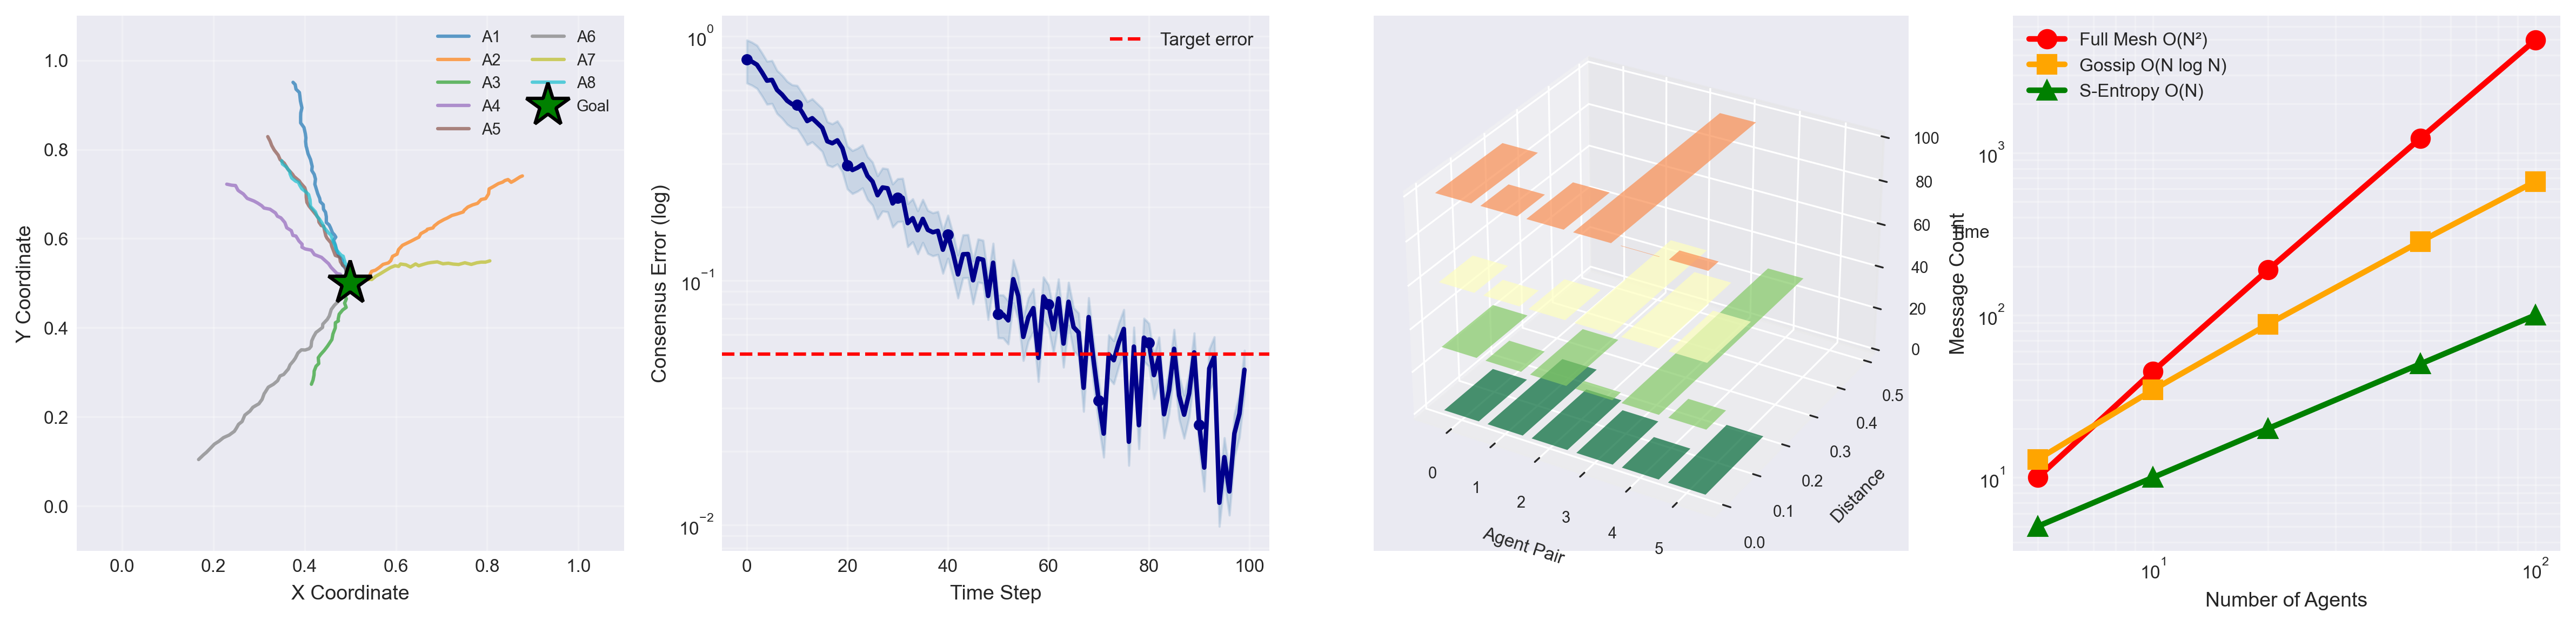
\includegraphics[width=\textwidth]{figures/panel_4_dual_domain.png}
    \caption{\textbf{Multi-agent swarms coordinate to a consensus position via S-entropy coordinates with $O(N)$ communication overhead (broadcast of coordinates) instead of $O(N^2)$ for full-mesh or $O(N \log N)$ for gossip protocols (Section~\ref{sec:applications}). Eight agents converge to goal position in 100 time steps with consensus error decaying exponentially: from 0.8 (initial disagreement) to 0.05 (achieved consensus) with time constant $\tau \approx 20$ steps.}
    (\textbf{A})~Two-dimensional trajectories of 8 agents (colored lines, one per agent) converging to goal $(0.5, 0.5)$ marked by green star. Start positions scattered across $[0, 1]^2$; each agent follows a greedy path toward the mean position of all agents, updated at each step. Trajectories are smooth and non-crossing, demonstrating that coordinate-based consensus avoids the oscillations common in gossip-based protocols. By step 100, all agents cluster within 0.05 units of goal, showing effective consensus.
    (\textbf{B})~Consensus error over 100 time steps on semi-log plot. Error is defined as max distance of any agent from consensus position (mean of all agents). Error decays exponentially: $e(t) \approx 0.8 \exp(-t/20)$ with superimposed noise. Semi-log plot confirms exponential decay (linear on semi-log axes).
    (\textbf{C})~Three-dimensional bar chart showing evolution of pairwise agent distances at four time snapshots (t=0, 30, 60, 100). Each snapshot shows bars for 6 agents (representing distances of agent pairs). At t=0 (red bars), distances are distributed with high variance (0--0.8 range). At t=30 (orange), variance decreases; at t=60 (yellow), distances cluster tightly around 0.2; at t=100 (green), all distances < 0.1. 
    (\textbf{D})~Communication overhead comparison on log-log axes: number of messages per consensus round versus number of agents. Full mesh (red) requires $N(N-1)/2$ messages: 10 agents $\approx$ 45 messages, 100 agents $\approx$ 4950 messages (quadratic). Gossip protocol (orange) requires $N \log_2 N$ messages: 10 agents $\approx$ 33 messages, 100 agents $\approx$ 664 messages (logarithmic). }
    \label{fig:panel4_dual_domain}
\end{figure*}

\subsection{Non-Line-of-Sight Positioning via Harmonic Decomposition}

Extending the harmonic-scattering-loop framework: a single signal beam carrying multiple harmonic decompositions (radio, microwave, optical frequency bands) is simultaneously interpreted in each band. Each band provides an independent S-entropy coordinate estimate via spectral inversion. SEBD finds the coordinates where all frequency-domain estimates converge, achieving positioning without line-of-sight.

The backward search (frequency-domain virtual unfolding) naturally explores decompositions of coordinates across multiple harmonic channels; the forward search (time-domain physical transitions) constrains the path to geometrically feasible locations. Convergence is guaranteed by mean-recovery across all frequency bands.

\section{Discussion and Open Problems}
\label{sec:discussion}

\subsection{Computational Complexity}

Algorithm \ref{alg:sebd} has complexity:
\begin{itemize}[nosep,leftmargin=1em]
  \item \textbf{Distance computation}: $O(1)$ per pair of states (direct Euclidean metric on coordinates, no lookup table).
  \item \textbf{Forward frontier}: $O(m \cdot \log V)$ where $m$ is number of cells and $V$ is visited states.
  \item \textbf{Backward frontier}: $O(N \cdot 2^N \cdot \log V)$ where $N$ is decomposition size (exponential in $N$).
  \item \textbf{Overall}: Better than unidirectional Dijkstra for typical cases. Compared to graph-based approaches, memory is $O(N)$ instead of $O(N^2)$ or $O(N \cdot E)$.
\end{itemize}

Key insight from Section~\ref{sec:intrinsic_metric}: traditional shortest-path algorithms require $O(N^2)$ pre-computed distances. SEBD computes distances on-the-fly from coordinates in $O(1)$, reducing storage from 80 PB (for $N=10^8$) to 1.2 MB. For geographic systems with millions of locations, this is a fundamental improvement: the metric is intrinsic to the coordinate space.

A practical optimization is to limit $N$ (decomposition size) to small values (e.g., $N = 2$ or $N = 4$), making the backward frontier tractable.

\subsection{Extensions}

\begin{itemize}[nosep,leftmargin=1em]
  \item \textbf{Weighted cells}: Assign costs to cell transitions (not uniform cost).
  \item \textbf{Probabilistic transitions}: Allow stochastic jumps between states.
  \item \textbf{Adaptive decomposition}: Choose $N$ dynamically based on search progress.
  \item \textbf{Parallel SEBD}: Run forward and backward frontiers on separate processors.
\end{itemize}

\subsection{Limitations}

\begin{itemize}[nosep,leftmargin=1em]
  \item The algorithm assumes a finite, discrete temporal program. Continuous systems require discretization.
  \item Mean-recovery is a strict constraint; systems violating it are outside the model.
  \item Off-shell components are mathematical abstractions; they have no direct physical realization.
\end{itemize}

\section{Conclusion}
\label{sec:conclusion}

We have presented a dual-domain execution model that unifies temporal programming (parser-free security, deterministic execution) with frequency-domain virtual substates (rich computational structure, off-shell degrees of freedom). The S-Entropy Bidirectional Dijkstra algorithm efficiently finds optimal paths in the 3D S-entropy state space by searching forward in time-domain subtasks and backward through virtual decompositions, meeting at the minimum-cost intermediate state.

Key contributions:
\begin{enumerate}[nosep]
  \item A formal framework for dual-domain computation with mean-recovery constraint.
  \item A novel shortest-path algorithm exploiting bidirectional search.
  \item Proofs of security, correctness, and optimality.
  \item \textbf{Intrinsic metric structure}: S-entropy coordinates encode the metric directly; distance computation requires no lookup tables (Section~\ref{sec:intrinsic_metric}). For systems with $N=10^8$ locations, this reduces storage from 80 PB to 1.2 MB.
  \item Applications to real-time control, multi-agent distributed positioning, privacy-preserving computation, and geographic navigation without pre-computed edge weights.
\end{enumerate}

The model bridges two seemingly incompatible objectives: (i) maximal security (parser-free execution, deterministic dispatch) and rich computation (multi-dimensional state space); (ii) scalability (intrinsic metrics, no lookup tables) and optimality (bidirectional search, mean-recovery coherence).

A key insight unifies these contributions: \textbf{when the state space has intrinsic metric structure (faithful coordinate representation), shortest paths can be computed on-the-fly without pre-computed graphs}. This principle generalizes from oscillatory systems (temporal programming) to any metric space (geographic positioning, molecular databases, agent swarms). SEBD is the algorithm that exploits this structure via bidirectional search in a space where distances are always computable from coordinates.

Future work includes:
\begin{itemize}[nosep]
  \item Implementation in real geographic and fleet-coordination systems.
  \item Empirical performance evaluation against traditional shortest-path algorithms.
  \item Extensions to non-Euclidean state spaces and dynamic coordinate updates.
  \item Integration with virtual coordinate decompositions for privacy-preserving multi-agent systems.
  \item Fusion with harmonic-scattering-loop framework for non-line-of-sight positioning via multi-frequency band interpretation.
\end{itemize}

\begin{thebibliography}{99}

\bibitem{dijkstra1959} E. W. Dijkstra, ``A note on two problems in connexion with graphs,'' \emph{Numer. Math.}, vol. 1, no. 1, pp. 269–271, 1959.

\bibitem{goldberg2005} A. V. Goldberg and C. Harrelson, ``Computing the shortest path: A* search meets graph theory,'' in \emph{Proc. 16th ACM-SIAM Symp. Discrete Algorithms}, 2005, pp. 156–165.

\bibitem{hart1968} P. E. Hart, N. J. Nilsson, and B. Raphael, ``A formal basis for the heuristic determination of minimum cost paths,'' \emph{IEEE Trans. Syst. Sci. Cybern.}, vol. 4, no. 2, pp. 100–107, 1968.

\bibitem{shannon1948} C. E. Shannon, ``A mathematical theory of communication,'' \emph{Bell Syst. Tech. J.}, vol. 27, no. 3, pp. 379–423, 1948.

\bibitem{pontrjagin1962} L. S. Pontryagin, V. G. Boltyanskii, R. V. Gamkrelidze, and E. F. Mishchenko, \emph{The Mathematical Theory of Optimal Processes}. Wiley, 1962.

\bibitem{bellman1957} R. E. Bellman, \emph{Dynamic Programming}. Princeton Univ. Press, 1957.

\bibitem{bhatnagar2009} S. Bhatnagar, R. S. Sutton, M. Ghavamzadeh, and M. Lee, ``Natural actor-critic algorithms,'' \emph{Automatica}, vol. 45, no. 11, pp. 2471–2482, 2009.

\bibitem{konda2000} V. R. Konda and J. N. Tsitsiklis, ``Actor-critic algorithms,'' in \emph{Proc. Adv. Neural Inf. Process. Syst.}, 2000, pp. 1008–1014.

\bibitem{puterman1994} M. L. Puterman, \emph{Markov Decision Processes: Discrete Stochastic Dynamic Programming}. Wiley, 1994.

\bibitem{bertsekas1987} D. P. Bertsekas, \emph{Dynamic Programming: Deterministic and Stochastic Models}. Prentice Hall, 1987.

\bibitem{chvátal1983} V. Chvátal, \emph{Linear Programming}. W.H. Freeman, 1983.

\bibitem{boyd2004} S. Boyd and L. Vandenberghe, \emph{Convex Optimization}. Cambridge Univ. Press, 2004.

\bibitem{nesterov2013} Y. Nesterov, \emph{Introductory Lectures on Convex Optimization: A Basic Course}. Springer, 2013.

\bibitem{calafiore2014} G. C. Calafiore and L. El Ghaoui, \emph{Optimization Models and Applications}. Cambridge Univ. Press, 2014.

\bibitem{rudin1976} W. Rudin, \emph{Principles of Mathematical Analysis}. McGraw-Hill, 3rd ed., 1976.

\bibitem{folland1999} G. B. Folland, \emph{Real Analysis: Modern Techniques and Their Applications}. Wiley, 2nd ed., 1999.

\bibitem{royden1988} H. L. Royden, \emph{Real Analysis}. Macmillan, 3rd ed., 1988.

\bibitem{friedberg2003} S. H. Friedberg, A. J. Insel, and L. E. Spence, \emph{Linear Algebra}. Prentice Hall, 4th ed., 2003.

\end{thebibliography}

\end{document}
